\documentclass[tikz,border=5pt]{standalone}
\usepackage{tikz}
\begin{document}
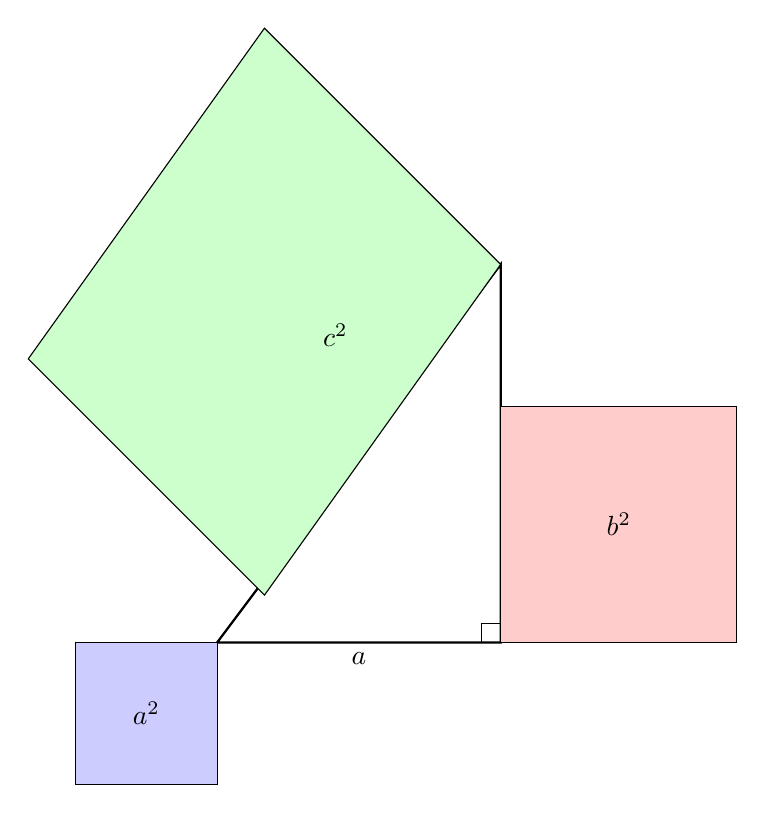
\begin{tikzpicture}[scale=1.2]
  % Right triangle
  \draw[thick] (0,0) -- (3,0) -- (3,4) -- cycle;
  \draw (2.8,0) -- (2.8,0.2) -- (3,0.2);
  
  % Labels
  \node[below] at (1.5,0) {$a$};
  \node[right] at (3,2) {$b$};
  \node[above left] at (1.5,2) {$c$};
  
  % Squares on sides
  \draw[fill=blue!20] (0,0) rectangle (-1.5,-1.5) node[midway] {$a^2$};
  \draw[fill=red!20] (3,0) rectangle (5.5,2.5) node[midway] {$b^2$};
  \draw[fill=green!20] (3,4) -- (0.5,6.5) -- (-2,3) -- (0.5,0.5) -- cycle;
  \node at (1.25,3.25) {$c^2$};
\end{tikzpicture}
\end{document}
